%%%%%%%%%%%%%%%%%%%%%%%%%%%%%%%%%%%%%%%%%%
\section{I principali canali di produzione}\label{ch:channels}
Andando ad analizzare invece quali siano i canali che producono più deuteroni, si è andati \textit{in primis} a riempire gli istogrammi relativi alle particelle di partenza, ossia si è andato a vedere per ogni deuterone prodotto quali siano le loro particelle madri.
Per semplificare la nomenclatura, prendendo in considerazione la \autoref{tab:canali}, chiameremo i canali (1-4) "canali $pn$", i canali (5-6) "canali $pp$" e i canali (7-8) "canali $nn$".
Lo stesso vale per gli antideuteroni con canali $\bar p\bar n$, $\bar p\bar p$ e $\bar n\bar n$.
Da ciò abbiamo tre distribuzioni per i deuteroni e tre per gli antideuteroni, rispettivamente con i canali $pn$, $pp$, $nn$ e $\bar p\bar n$, $\bar p\bar p$, $\bar n\bar n$.
In \autoref{fig:A_ov_deut} e in \autoref{fig:A_ov_antideut} vengono riportate le distribuzioni di questi canali in sovrapposizione, mentre in \autoref{fig:A_ov_stack_deut} e in \autoref{fig:A_ov_stack_antideut} viene riportata la produzione relativa di (anti)deuteroni.  
Si può osservare che \pythiaa{} assegna a ognuno di questi canali uno stesso peso nella produzione sia deuteronica e sia antideuteronica, se non per un piccolo incremento per il canale $pn$ nei deuteroni e il canale $\bar p\bar n$ negli antideuteroni.\\

Successivamente si è andati ad analizzare la produzione relativa dei subcanali dei canali $pn$, $pp$ e $nn$ e delle relative antiparticelle, andando a vedere quali siano i loro principali contributi.
In \autoref{fig:A_deut_subchannels} e in \autoref{fig:A_antideut_subchannels} possiamo osservare tali contributi.
Si nota che il contributo più abbondante per tutti e sei i canali è quello in cui avviene la produzione di un (anti)deuterone e di un pione, mentre il contributo minore nella produzione è la cattura radiativa.
Invece la produzione di un deuterone e di due pioni è meno abbondante, perché essa richiede più energia ed è meno probabile che avvenga.

È curioso notare che in \autoref{fig:A_pn_stack_deut} e in \autoref{fig:A_pn_stack_antideut} il processo $pn\to \pi^+\pi^- D$ ($ \bar p \bar n\to \pi^+\pi^- \bar D$) pare più abbondante del processo $pn\to \pi^0\pi^0D$ ($ \bar p \bar n\to \pi^0\pi^0 \bar D$).
Questo può essere spiegato con l'invarianza di isospin, per cui si ha che (\cite{Dal_2015})
\begin{equation}
    \sigma_{pn\to\pi^+\pi^-D} = 2\sigma_{pn\to\pi^0\pi^0D} + \dfrac12\sigma_{pp\to\pi^+\pi^0D}
\end{equation}
con $\sigma_\text{processo}$ la sezione d'urto del processo associato.
\begin{figure}[htbp]
    \centering
    \begin{subfigure}{.49\textwidth}
    \centering
        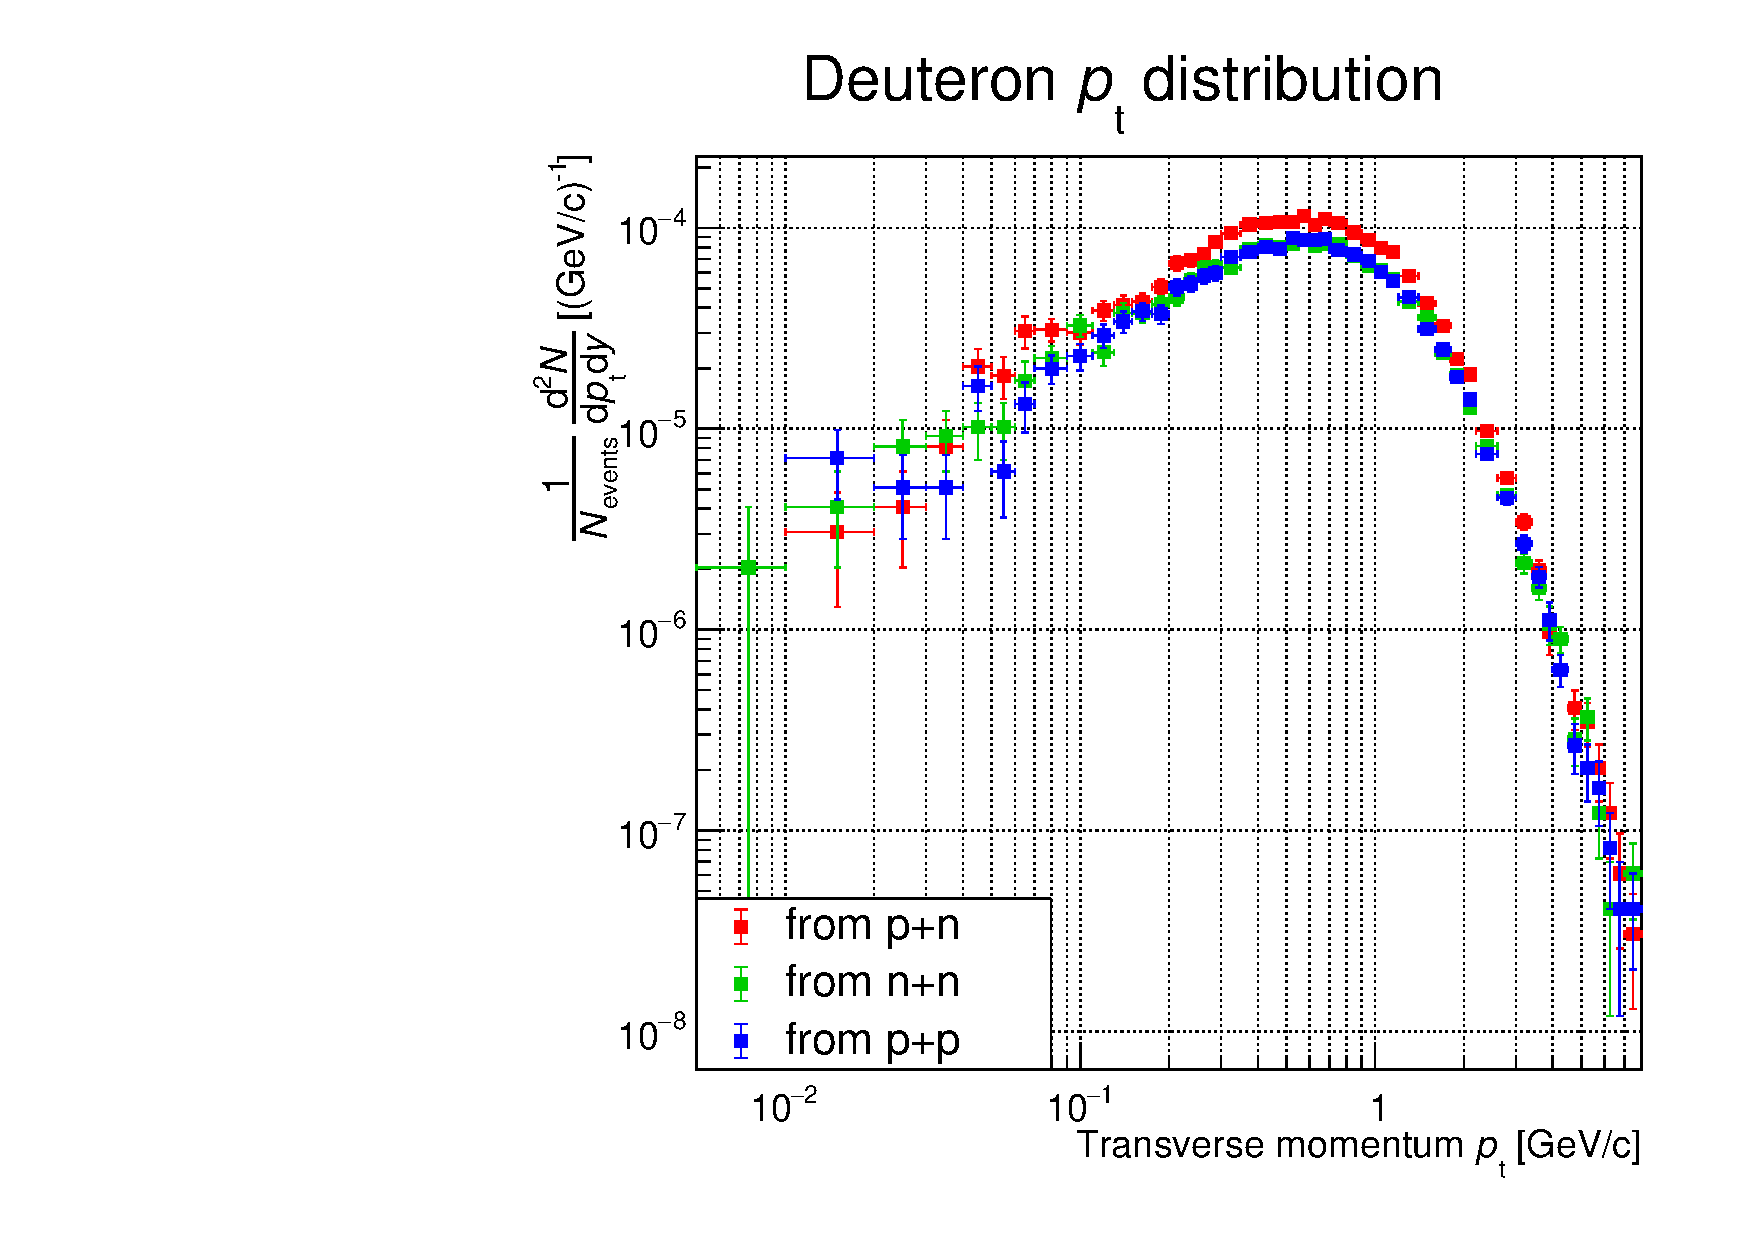
\includegraphics[width=\textwidth]{image/3-risultati/deuteron_analyse/A/ov_log.pdf}
        \caption{}
        \label{fig:A_ov_deut}
    \end{subfigure}
    %\hspace{1cm}
    \begin{subfigure}{.49\textwidth}
        \centering
        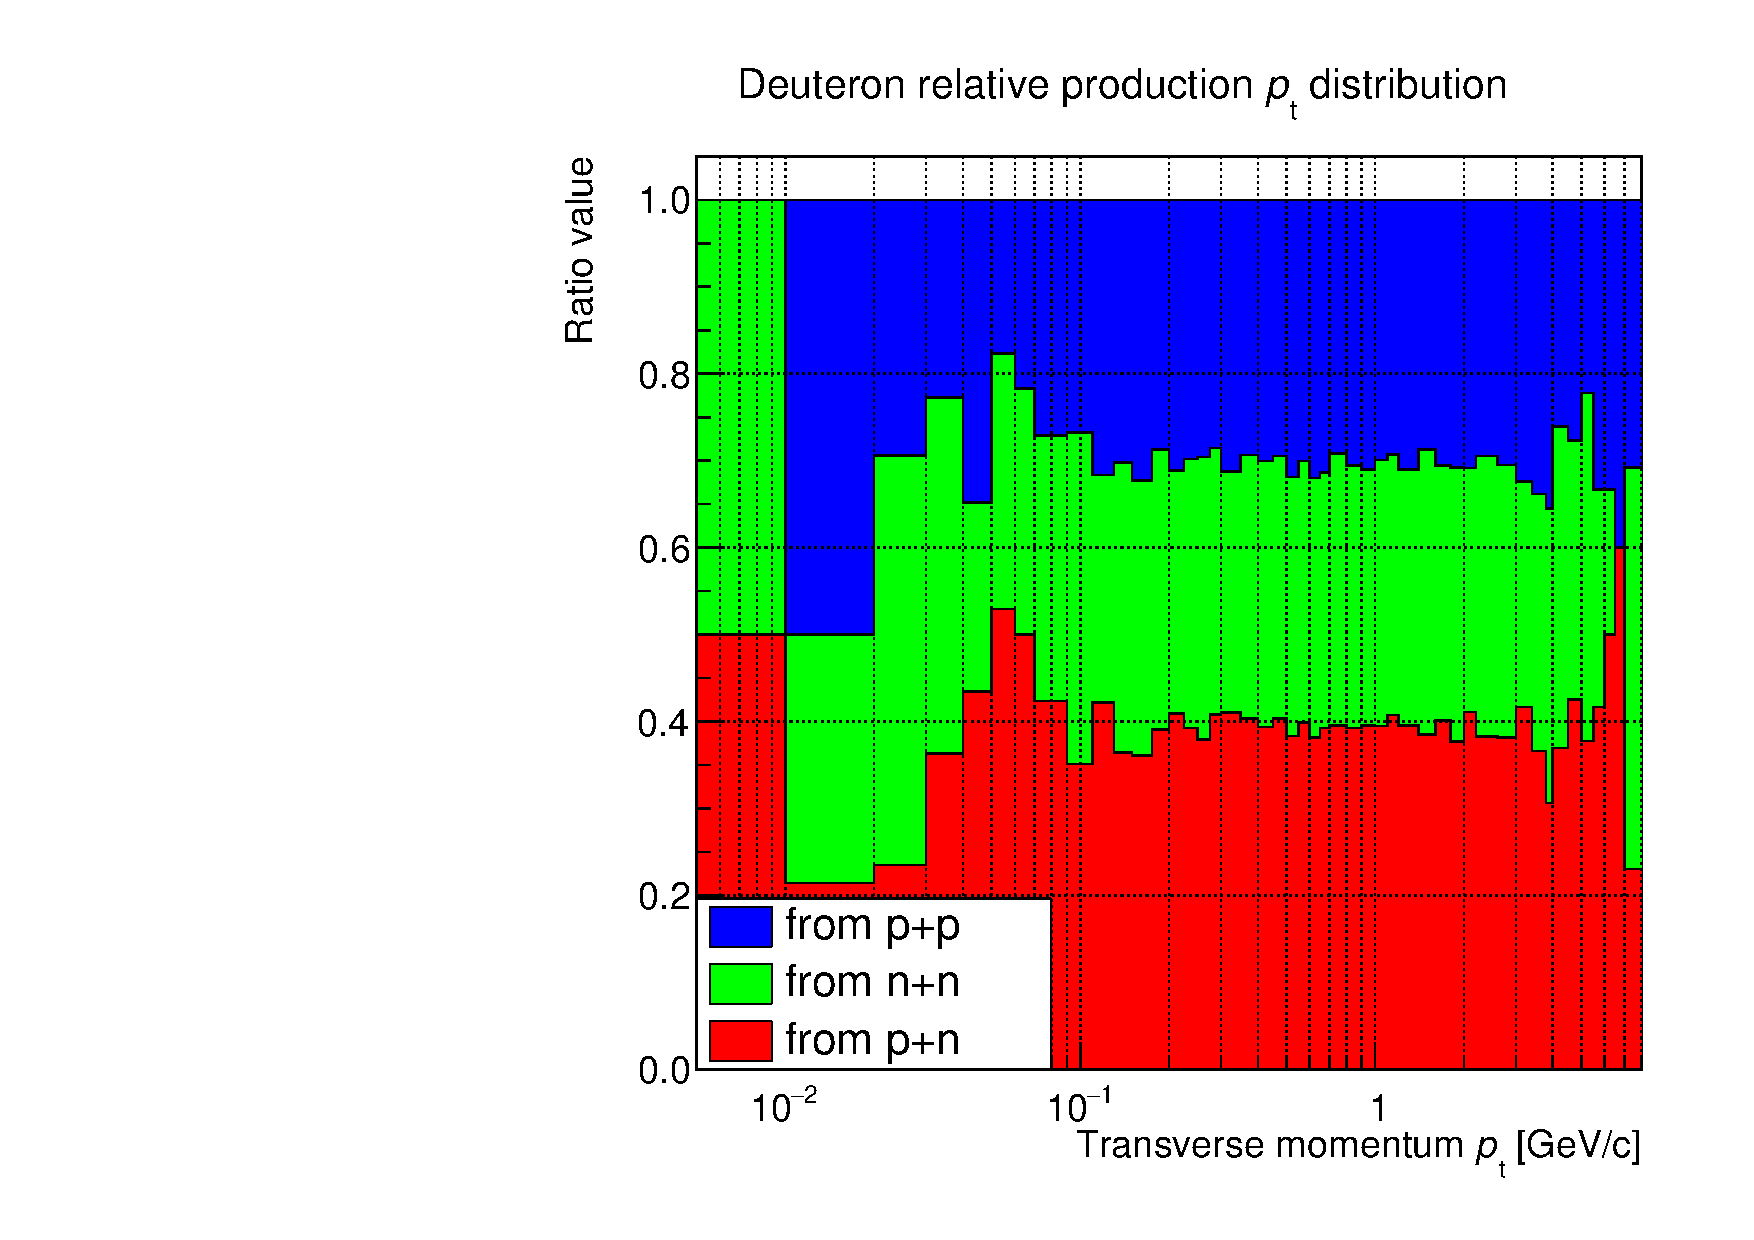
\includegraphics[width=\textwidth]{image/3-risultati/deuteron_analyse/A/ov_stack.pdf}
        \caption{}
        \label{fig:A_ov_stack_deut}
    \end{subfigure}
    \begin{subfigure}{.49\textwidth}
    \centering
        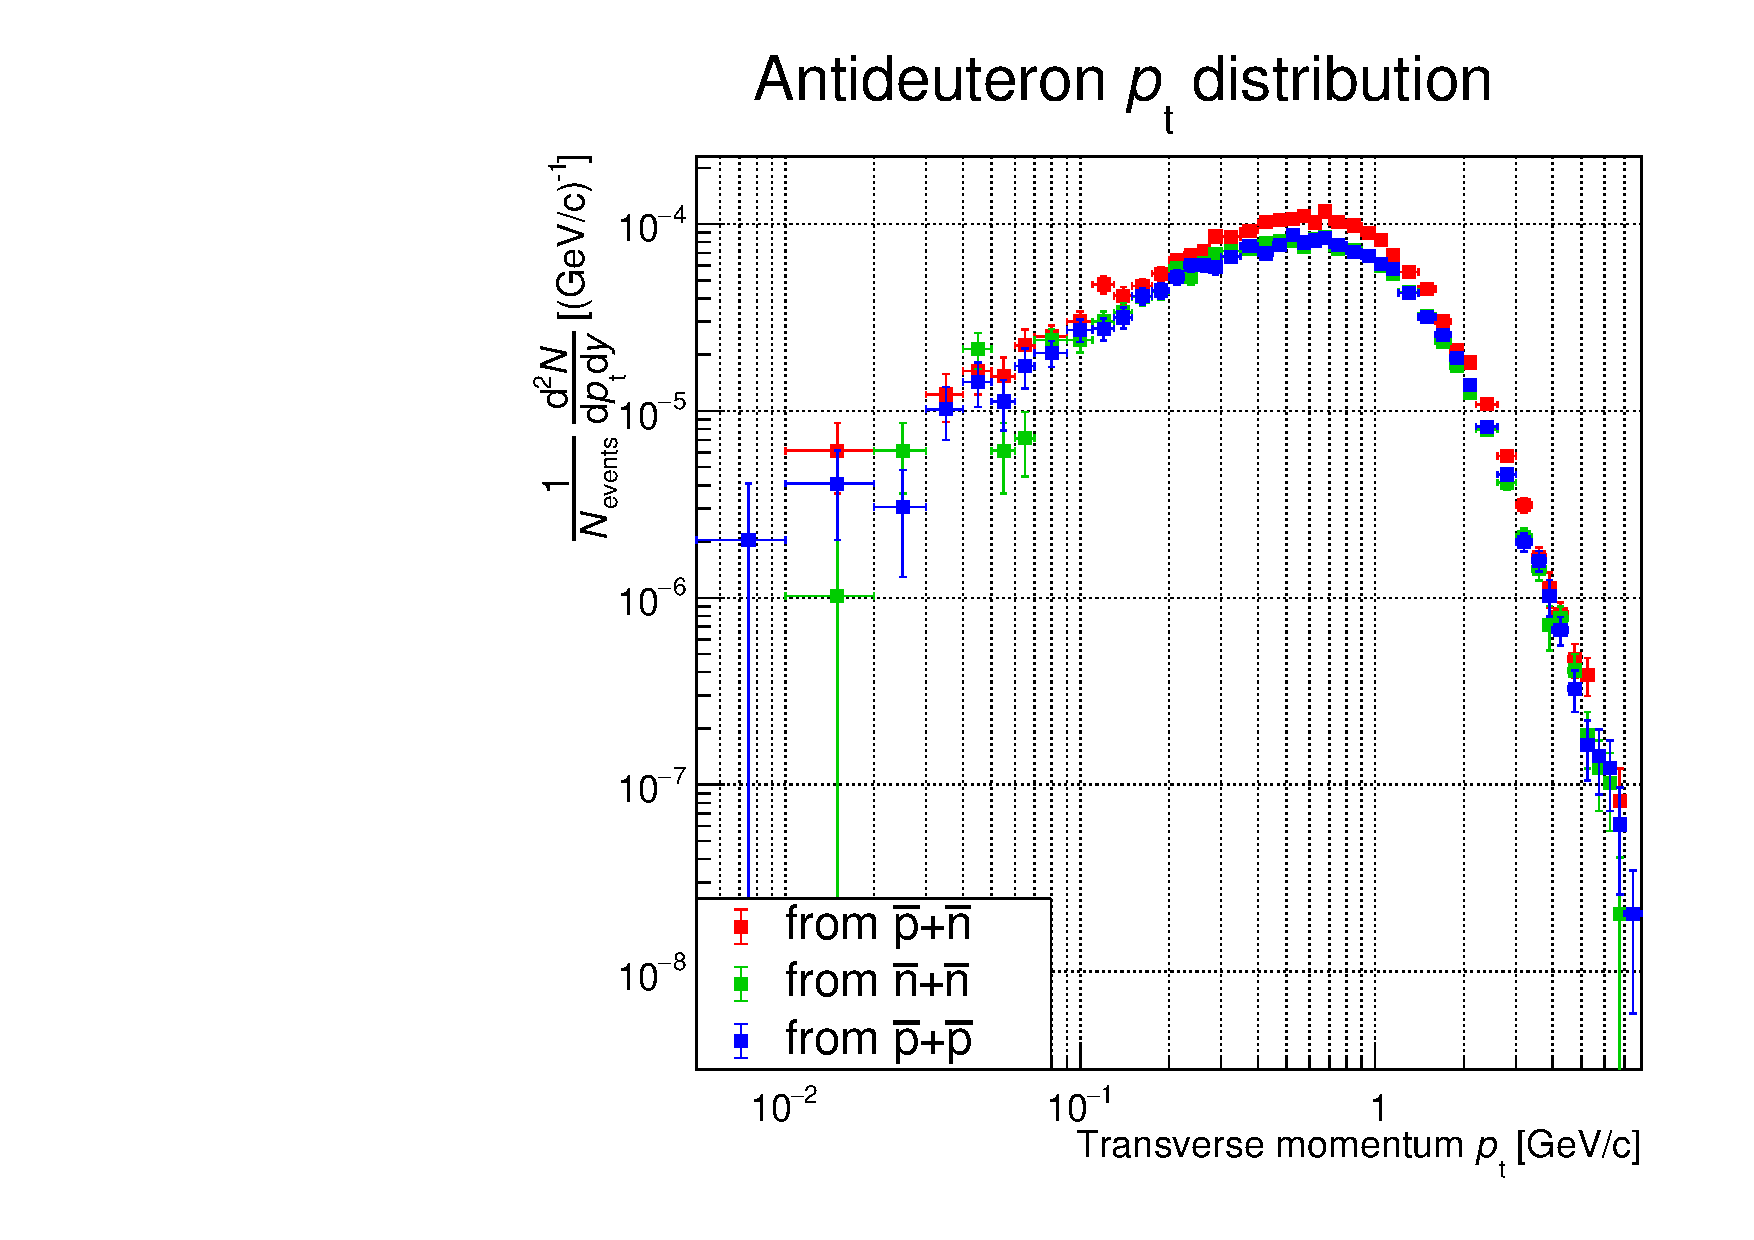
\includegraphics[width=\textwidth]{image/3-risultati/antideuteron_analyse/A/ov_log.pdf}
        \caption{}
        \label{fig:A_ov_antideut}
    \end{subfigure}
    %\hspace{1cm}
    \begin{subfigure}{.49\textwidth}
        \centering
        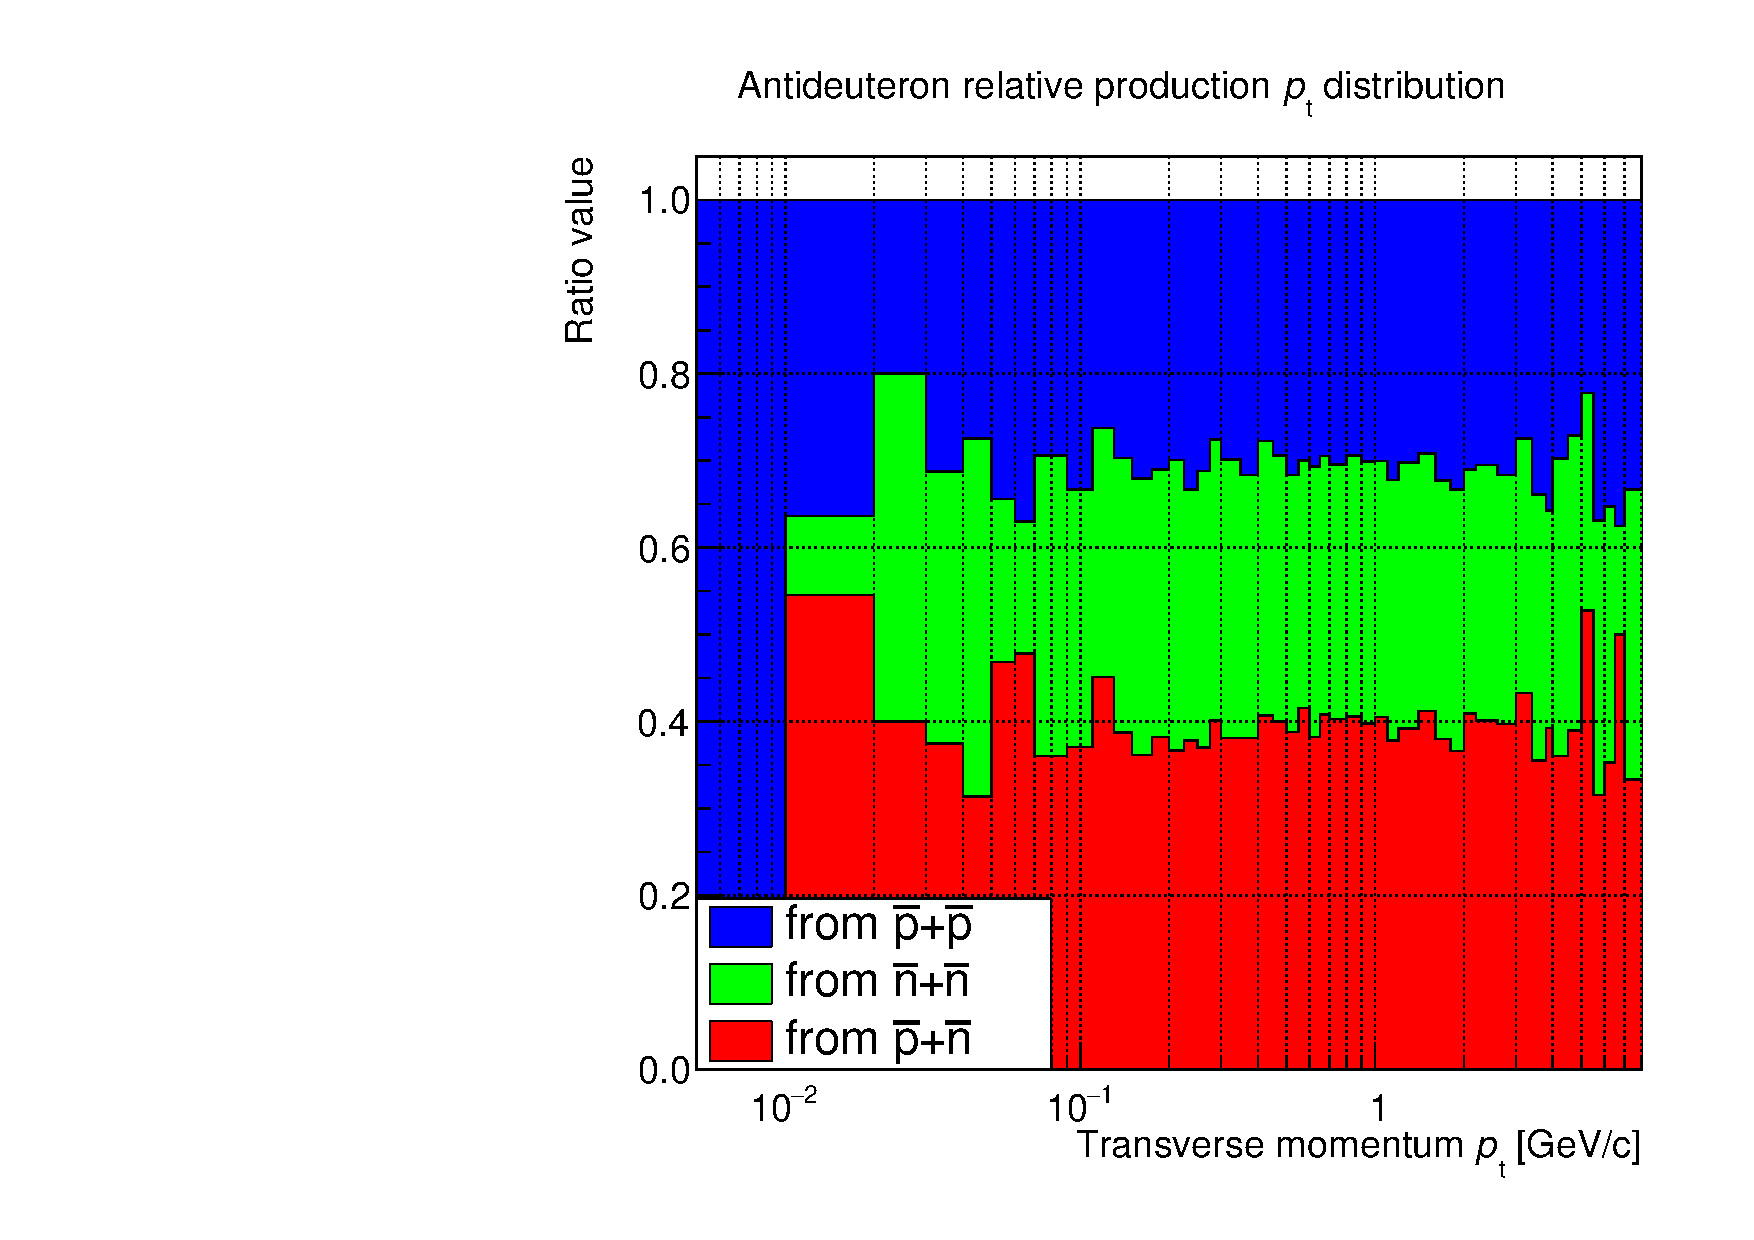
\includegraphics[width=\textwidth]{image/3-risultati/antideuteron_analyse/A/ov_stack.pdf}
        \caption{}
        \label{fig:A_ov_stack_antideut}
    \end{subfigure}
    \caption{\emph{\rmfamily (a)} Distribuzioni dell'impulso trasverso di $D$ dei canali $pn$, $pp$ e $nn$ e \emph{\rmfamily (b)} la produzione relativa nei vari canali di $D$. \emph{\rmfamily (c)} Distribuzioni dell'impulso trasverso di $\bar D$ dei canali $\bar p\bar n$, $\bar p\bar p$ e $\bar n\bar n$ e \emph{\rmfamily (d)} la produzione relativa nei vari canali di $\bar D$.}
    \label{fig:A_ov}
\end{figure}
\begin{figure}[htbp]
    \centering
    \begin{subfigure}{.49\textwidth}
    \centering
        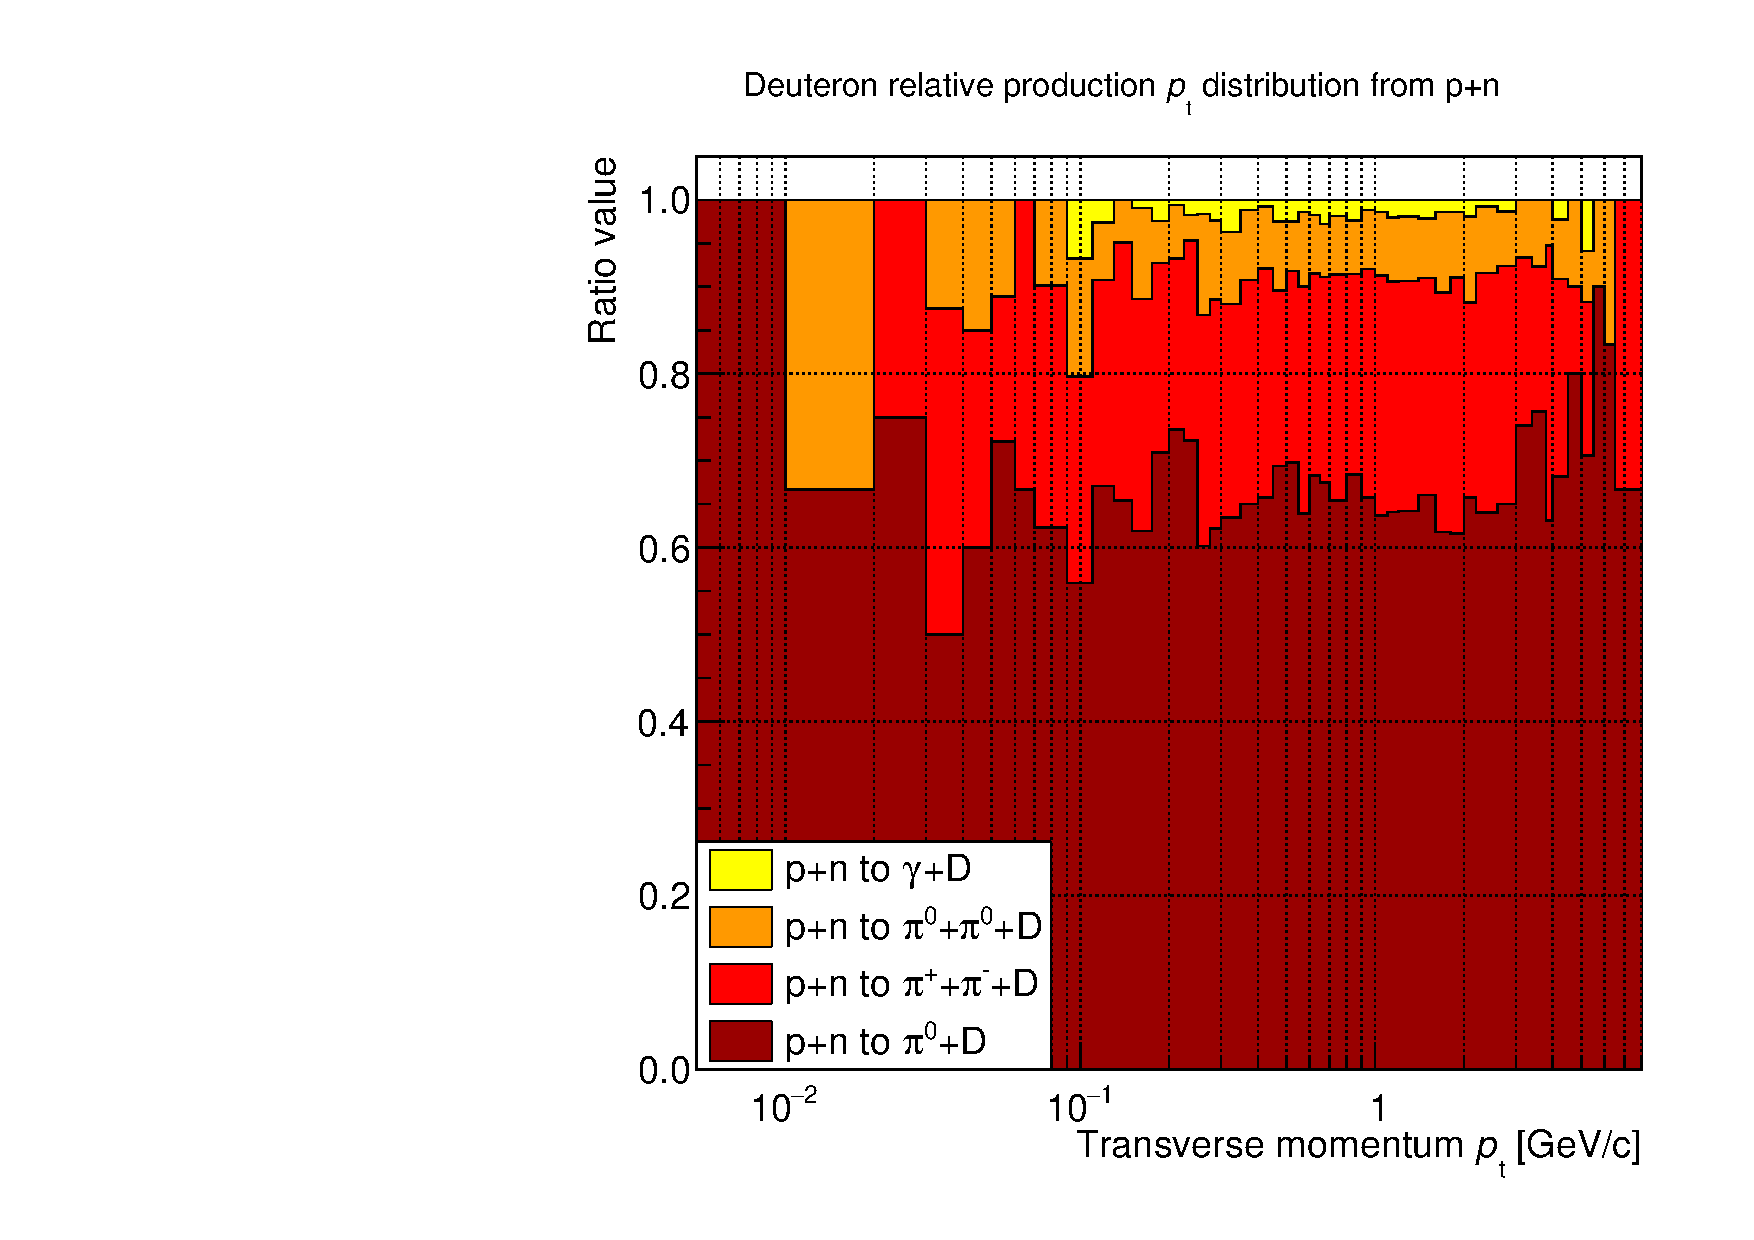
\includegraphics[width=\textwidth]{image/3-risultati/deuteron_analyse/A/p_n_stack.pdf}
        \caption{}
        \label{fig:A_pn_stack_deut}
    \end{subfigure}
    %\hspace{1cm}
    \begin{subfigure}{.49\textwidth}
        \centering
        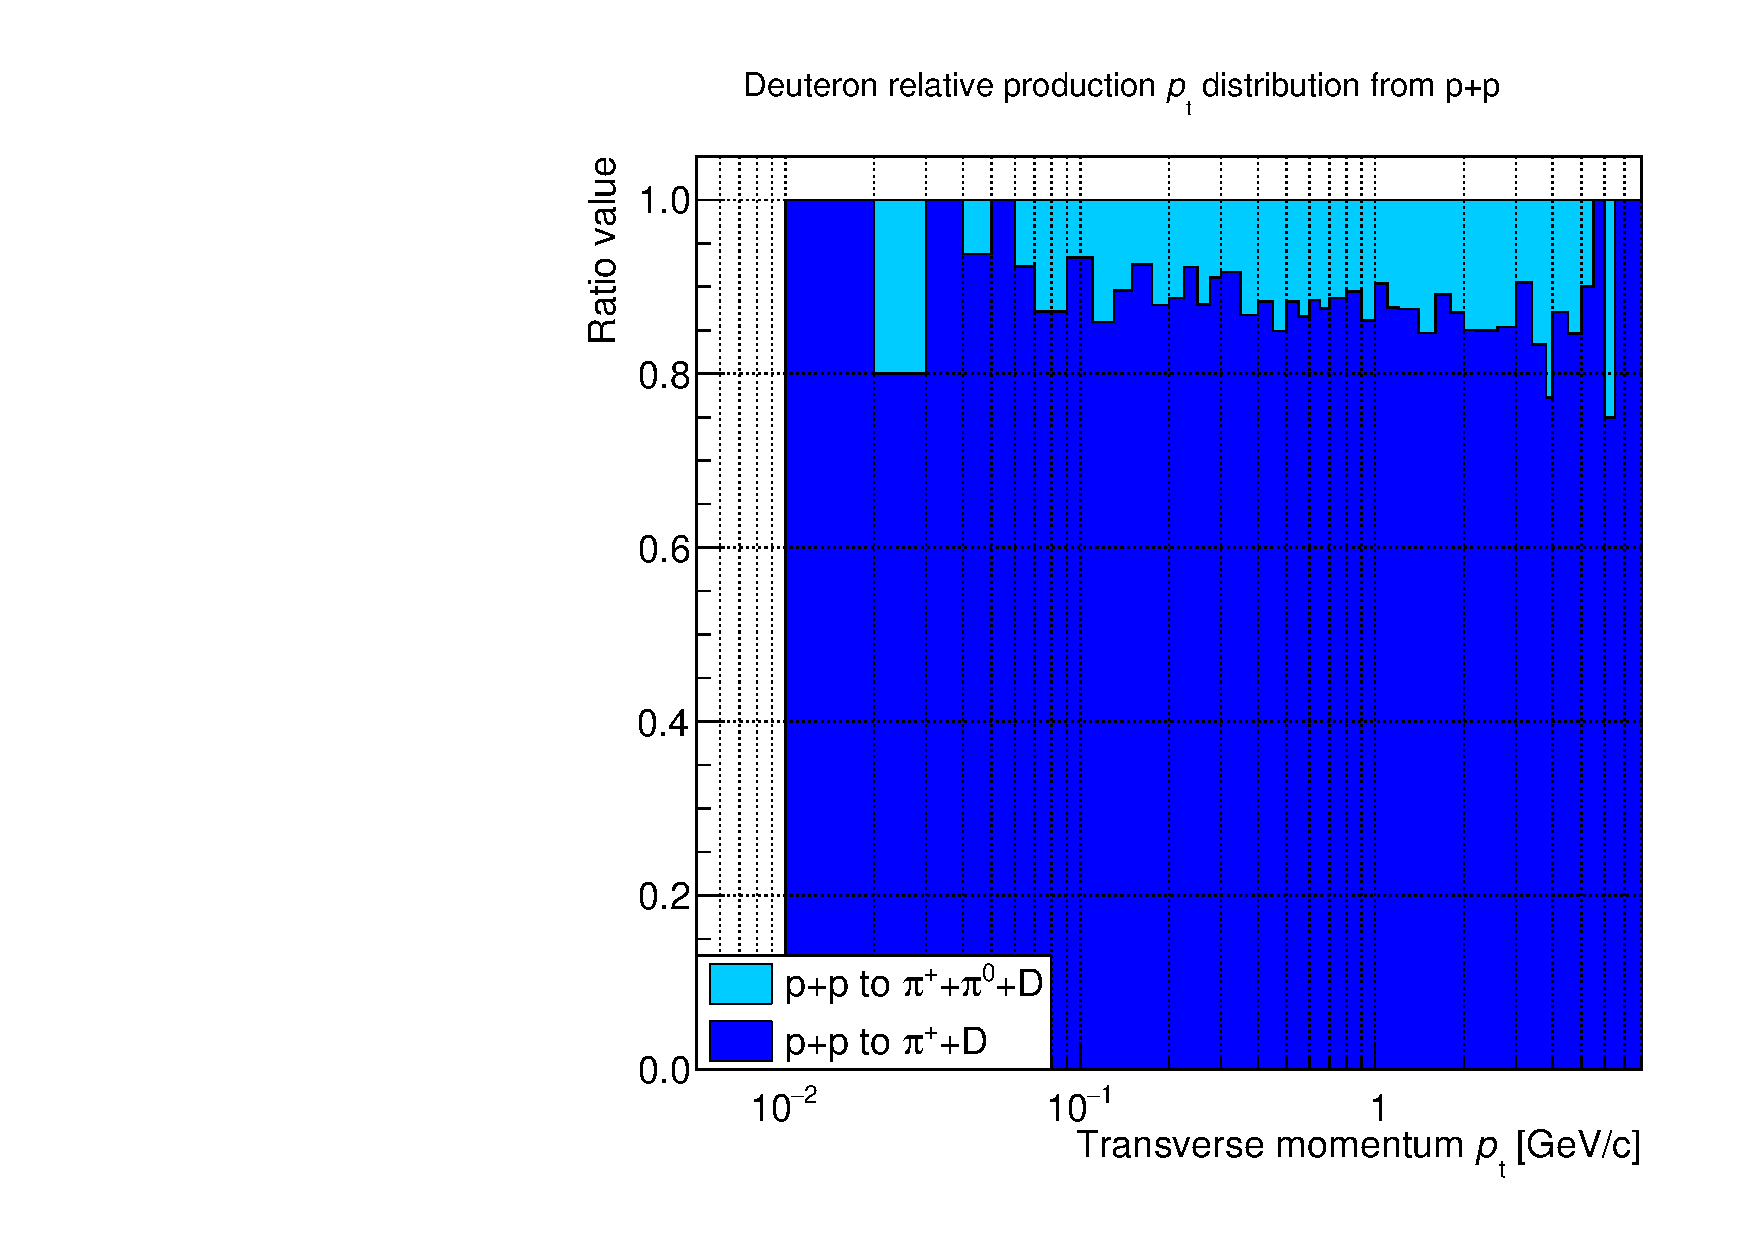
\includegraphics[width=\textwidth]{image/3-risultati/deuteron_analyse/A/p_p_stack.pdf}
        \caption{}
        \label{fig:A_pp_stack_deut}
    \end{subfigure}
    \begin{subfigure}{.49\textwidth}
    \centering
        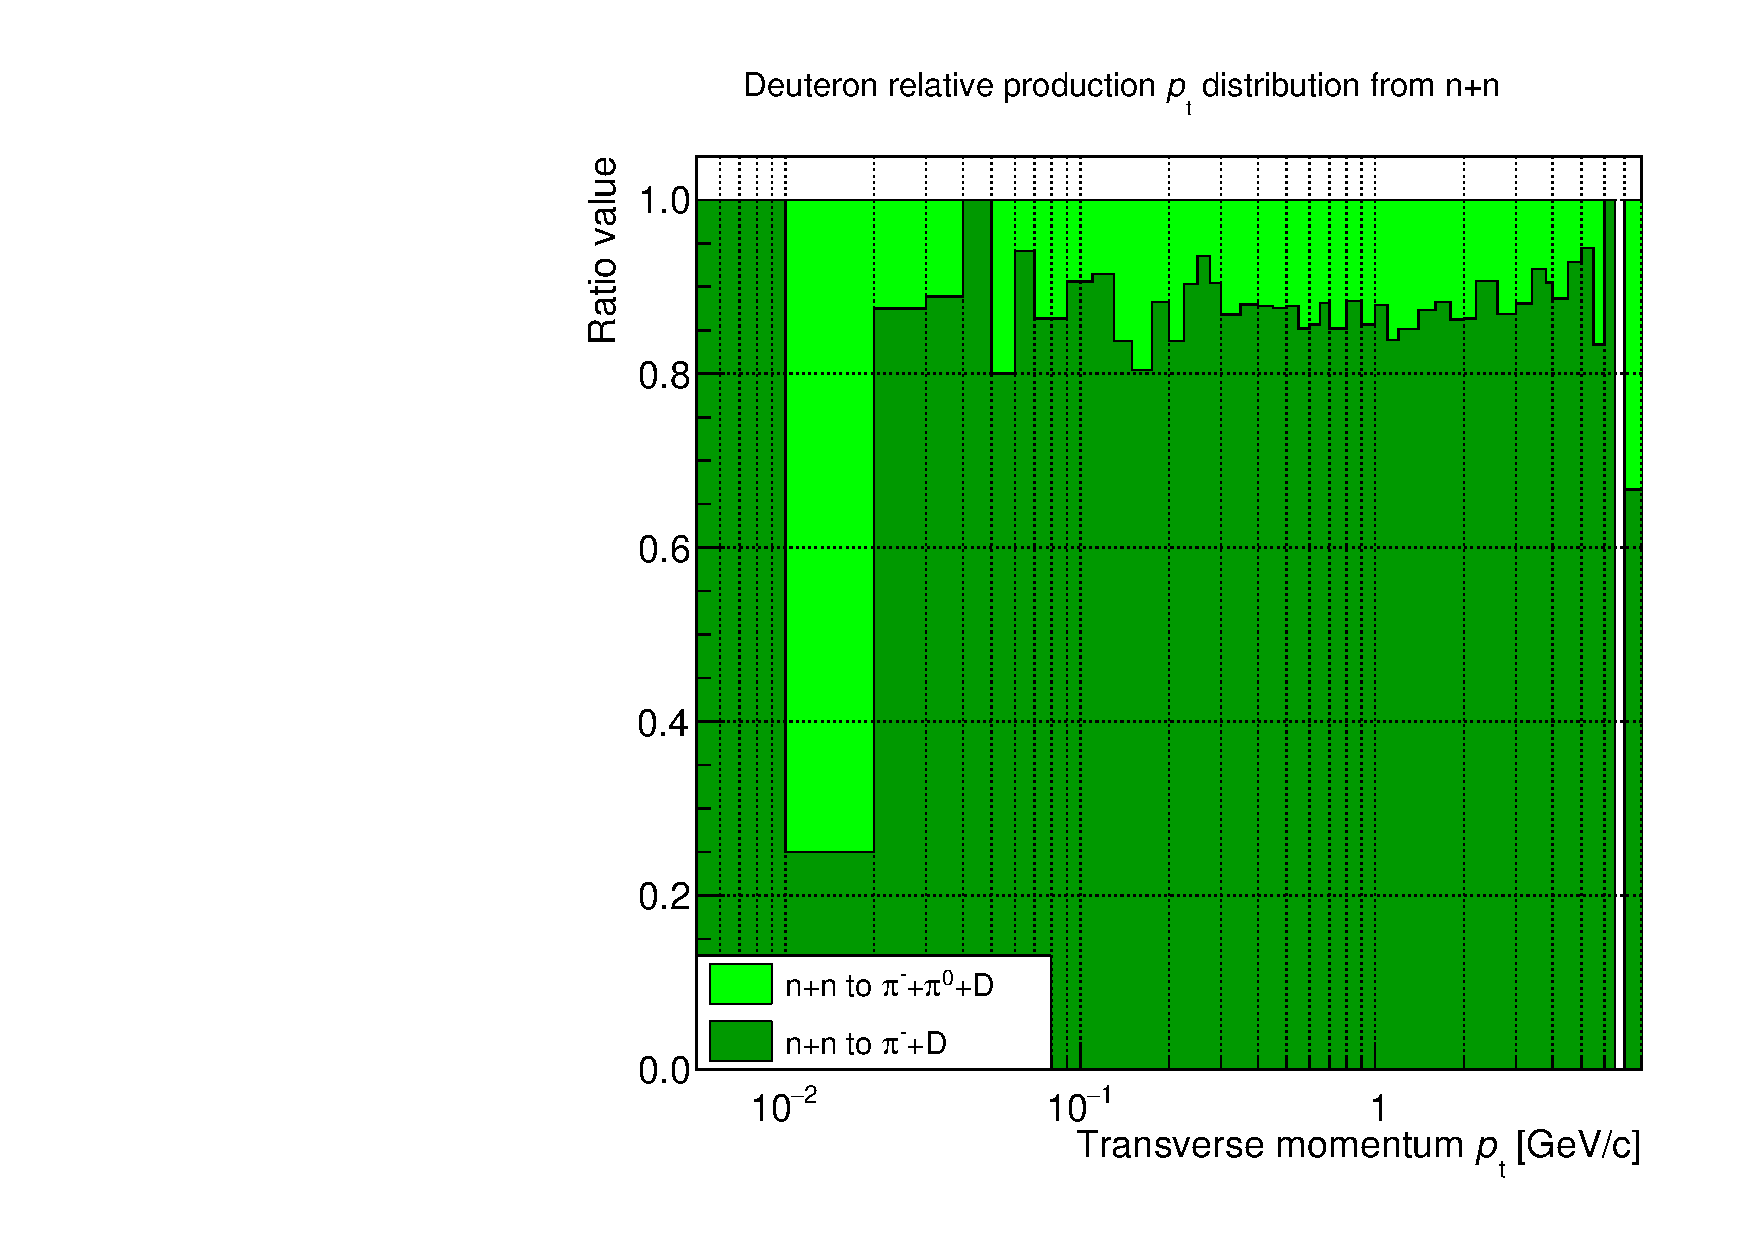
\includegraphics[width=\textwidth]{image/3-risultati/deuteron_analyse/A/n_n_stack.pdf}
        \caption{}
        \label{fig:A_nn_stack_deut}
    \end{subfigure}
    \caption{Produzione relativa di $D$ dei canali \emph{\rmfamily (a)} $pn$, \emph{\rmfamily (b)} $pp$ e \emph{\rmfamily (c)} $nn$.}
    \label{fig:A_deut_subchannels}
\end{figure}
\begin{figure}[htbp]
    \centering
    \begin{subfigure}{.49\textwidth}
    \centering
        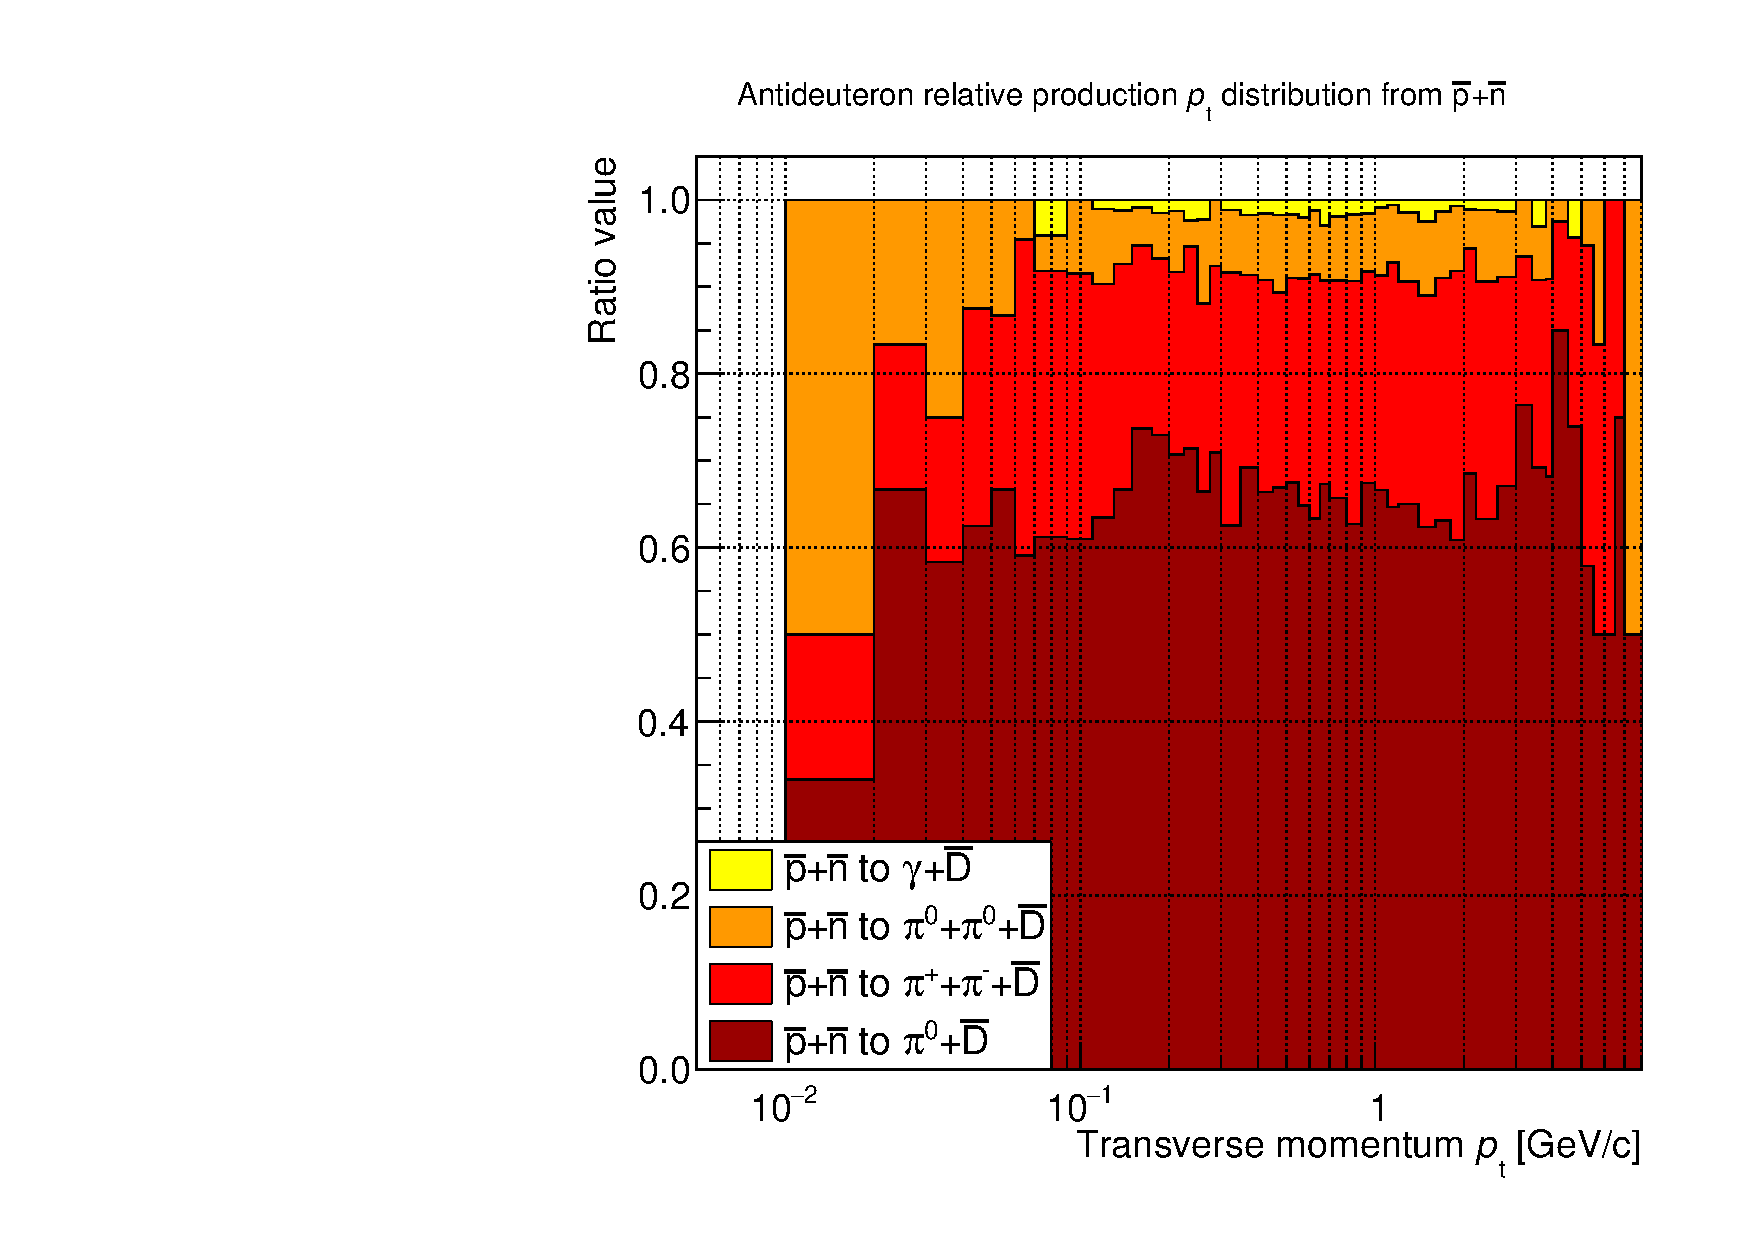
\includegraphics[width=\textwidth]{image/3-risultati/antideuteron_analyse/A/p_n_stack.pdf}
        \caption{}
        \label{fig:A_pn_stack_antideut}
    \end{subfigure}
    %\hspace{1cm}
    \begin{subfigure}{.49\textwidth}
        \centering
        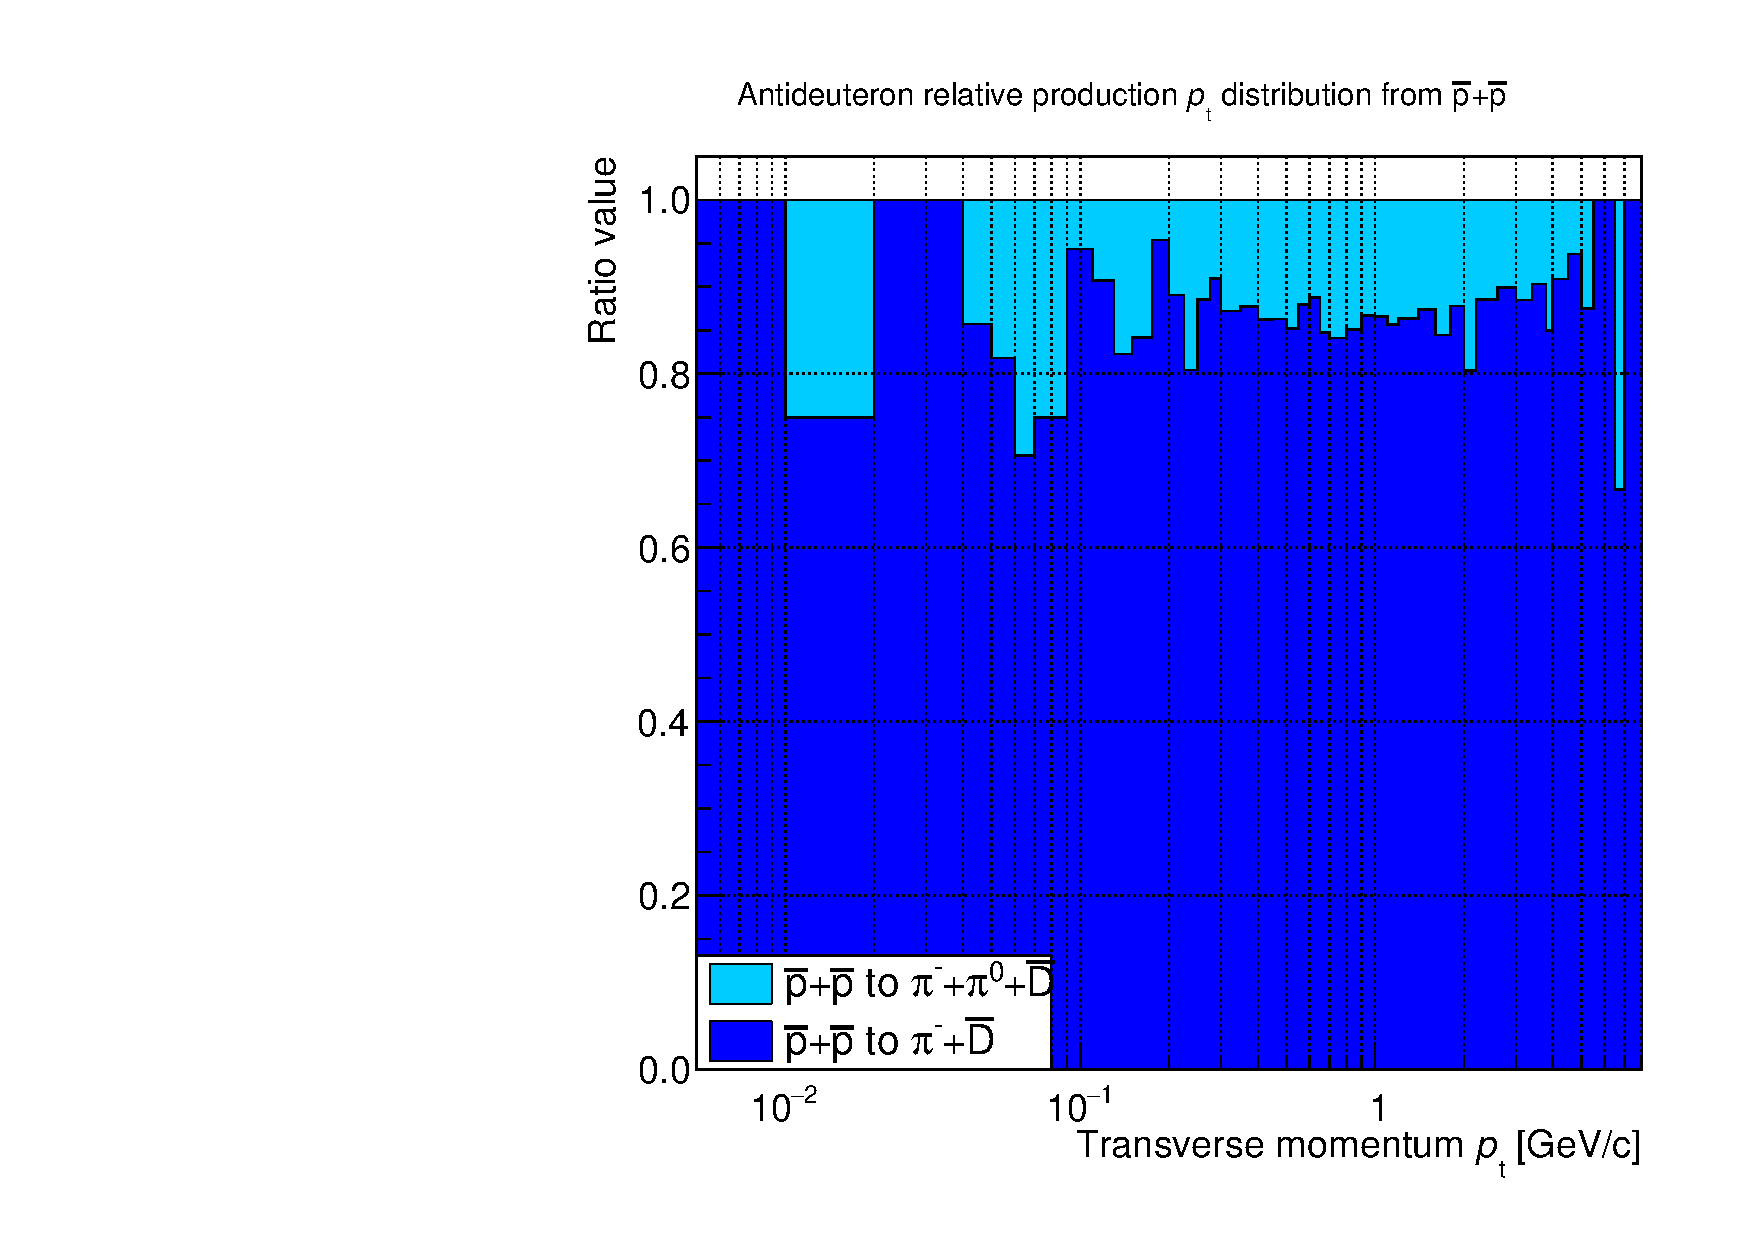
\includegraphics[width=\textwidth]{image/3-risultati/antideuteron_analyse/A/p_p_stack.pdf}
        \caption{}
        \label{fig:A_pp_stack_antideut}
    \end{subfigure}
    \begin{subfigure}{.49\textwidth}
    \centering
        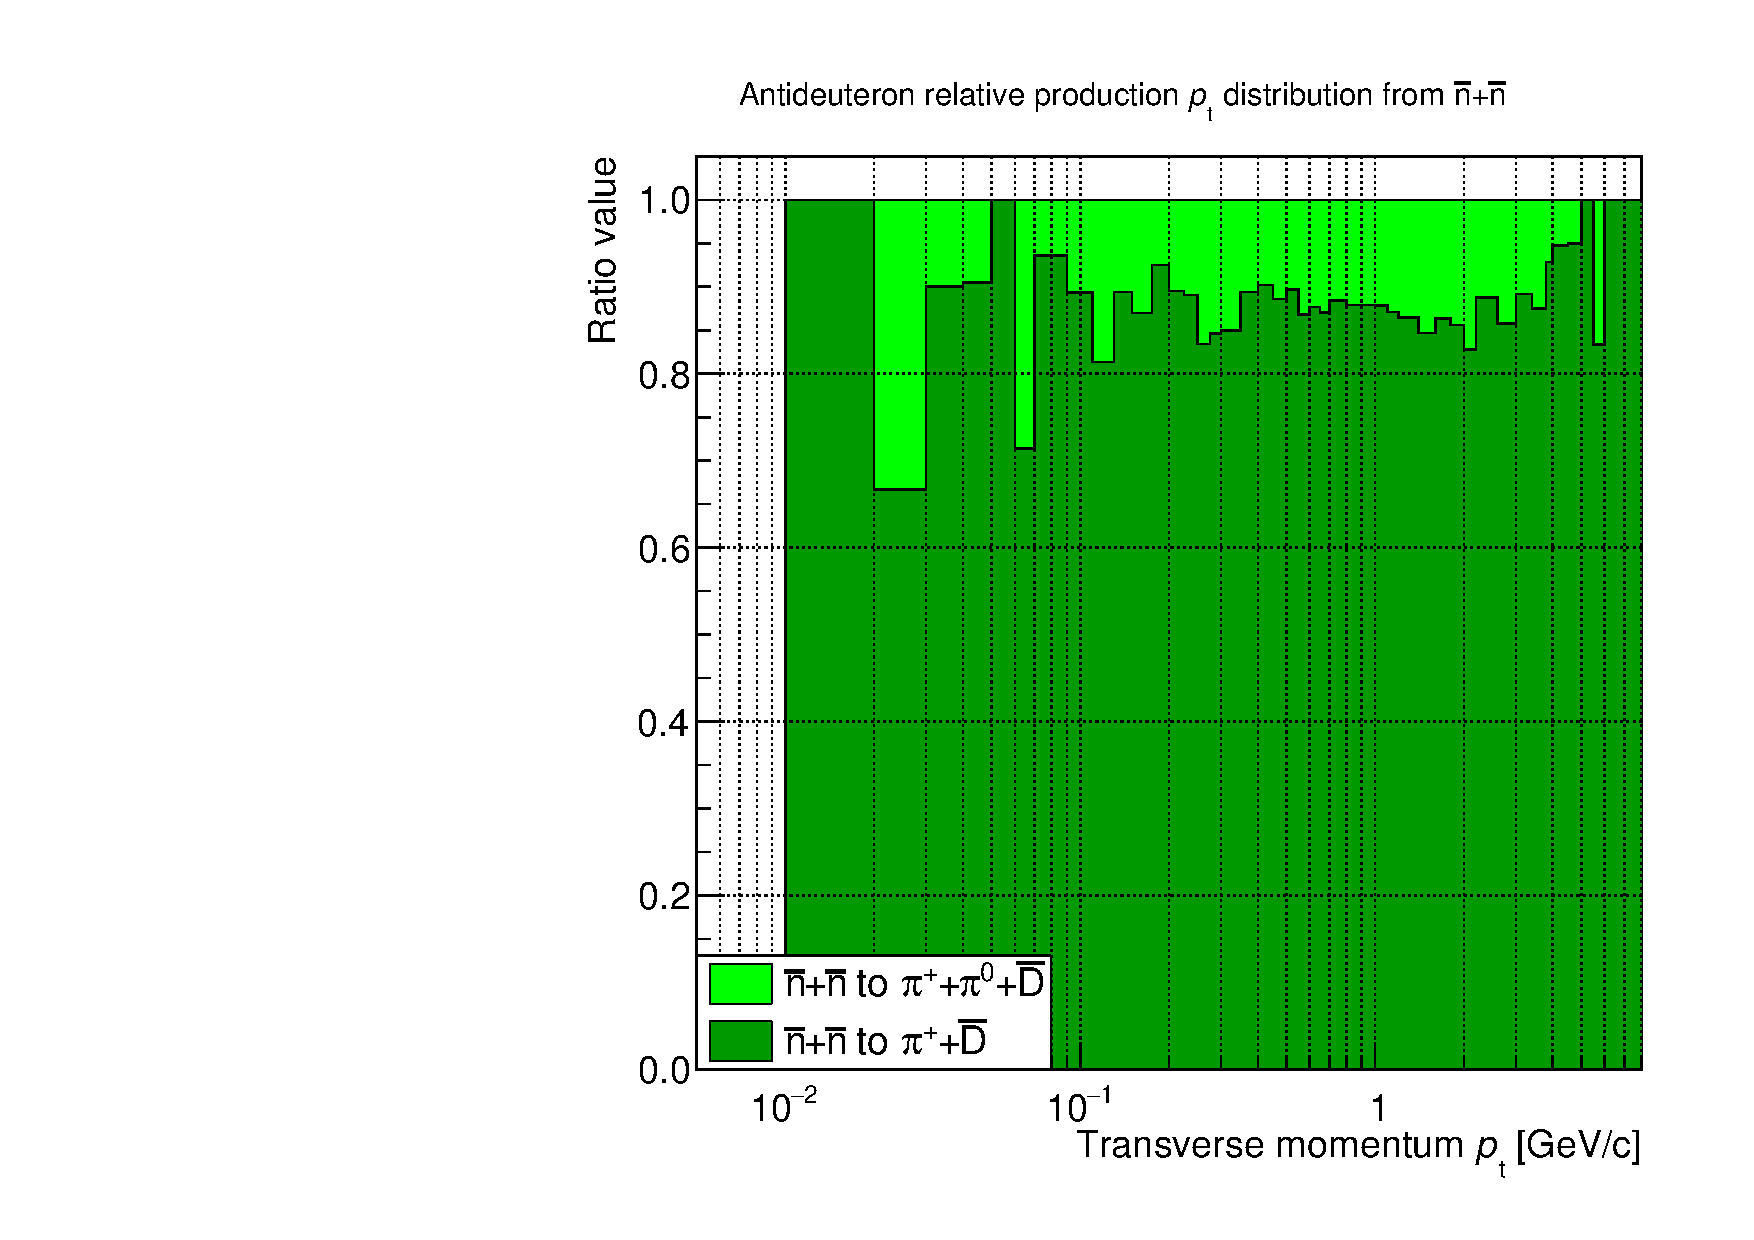
\includegraphics[width=\textwidth]{image/3-risultati/antideuteron_analyse/A/n_n_stack.pdf}
        \caption{}
        \label{fig:A_nn_stack_antideut}
    \end{subfigure}
    \caption{Produzione relativa di $\bar D$ dei canali \emph{\rmfamily (a)} $\bar p\bar n$, \emph{\rmfamily (b)} $\bar p\bar p$ e \emph{\rmfamily (c)} $\bar n\bar n$.}
    \label{fig:A_antideut_subchannels}
\end{figure}